\documentclass[10pt,twocolumn,letterpaper]{article}

% สิ่งที่ฉันเพิ่มเอง
\usepackage{booktabs}
% \usepackage{caption}
% \captionsetup[table]{skip=8pt}   % มีผลเฉพาะกับตาราง
\usepackage{stfloats}  % เพิ่มอันนี้ใน preamble
\usepackage{float}
\usepackage[T1]{fontenc}

\usepackage{babel}

\babelprovide[main,import,maparabic]{thai}

\babelfont{rm}{FreeSerif}

\usepackage{microtype}

\usepackage{cvpr}
\usepackage{times}
\usepackage{epsfig}
\usepackage{graphicx}
\usepackage{amsmath}
\usepackage{amssymb}


\usepackage[breaklinks=true,bookmarks=false]{hyperref}
\cvprfinalcopy % *** ยกเลิกคอมเมนต์บรรทัดนี้สำหรับการส่งต้นฉบับฉบับสุดท้าย

\makeatletter
\def\cvprsubsection{\@startsection {subsection}{2}{\z@}
    {8pt plus 2pt minus 2pt}{6pt}{\bfseries\normalsize}}
\makeatother


\def\cvprPaperID{****} % *** ใส่รหัสประจำตัวกระดาษ CVPR ที่นี่
\def\httilde{\mbox{\tt\raisebox{-.5ex}{\symbol{126}}}}

% หน้าถูกนับเลขในโหมดส่งต้นฉบับ และไม่มีเลขหน้าในฉบับกล้องพร้อมพิมพ์
%\ifcvprfinal\pagestyle{empty}\fi
\setcounter{page}{1}
\begin{document}

%%%%%%%%% TITLE
\title{บทปูพื้นฐานโดยขับเคลื่อนด้วยข้อมูลของ ECDO ภาค 1/2: ความเข้าใจปัจจุบันเกี่ยวกับทฤษฎีการแยกตัวคอร์และแมนเทิลแบบคายความร้อน Dzhanibekov Oscillation (ECDO) หรือ “Earth Flip”}

\author{จุนโฮ\\
เผยแพร่ กุมภาพันธ์ 2025\\
เว็บไซต์ (ดาวน์โหลดเอกสารที่นี่): \href{https://sovrynn.github.io}{sovrynn.github.io}\\
คลังวิจัย ECDO: \href{https://github.com/sovrynn/ecdo}{github.com/sovrynn/ecdo}\\
{\tt\small junhobtc@proton.me}
}
\maketitle
%\thispagestyle{empty}

\begin{abstract}
ในเดือนพฤษภาคม ค.ศ. 2024 ผู้เขียนนิรนามออนไลน์ชื่อว่า “The Ethical Skeptic” \cite{0} ได้แบ่งปันทฤษฎีใหม่ที่ปฏิวัติความคิด ชื่อว่า การแยกตัวของแกน-แมนเทิลด้วยปฏิกิริยาอุณหภูมิสูงร่วมกับการสั่นแบบ Dzhanibekov (Exothermic Core-Mantle Decoupling Dzhanibekov Oscillation - ECDO) \cite{1} ทฤษฎีนี้เสนอว่า โลกเคยประสบกับการเปลี่ยนแปลงอย่างฉับพลันของแกนหมุนโลก นำไปสู่น้ำท่วมขนาดใหญ่ทั่วโลกเมื่อมหาสมุทรไหลบ่าข้ามทวีปจากแรงเฉื่อยการหมุนของโลก นอกจากนี้ ยังมีการนำเสนอกระบวนการทางธรณีฟิสิกส์และข้อมูลที่บ่งชี้ว่า การสลับขั้วเช่นนี้อาจเกิดขึ้นอีกในไม่ช้า แม้การทำนายเหตุการณ์น้ำท่วมโลกและวันโลกาวินาศจะไม่ใช่เรื่องใหม่ แต่ทฤษฎี ECDO มีความน่าสนใจอย่างยิ่งเนื่องจากใช้วิธีการทางวิทยาศาสตร์ สมัยใหม่ สหสาขาวิชาชีพ และอ้างอิงข้อมูลจริง

บทความนี้เป็นส่วนแรกจากสองส่วนของบทสรุปย่อจากการวิจัยอิสระเป็นเวลาหกเดือน \cite{2,20} เกี่ยวกับทฤษฎี ECDO ซึ่งจะเน้นประเด็นสำคัญสามข้อดังนี้:

\begin{flushleft}
\begin{enumerate}
    \item ปรากฏการณ์ 'Earth flip' ที่คล้าย ECDO ได้เกิดขึ้นหลายครั้งในประวัติศาสตร์มนุษย์เมื่อไม่นานมานี้ ดังเห็นได้จากตำนานน้ำท่วมและร่องรอยทางธรณีวิทยาของน้ำท่วมข้ามทวีป
    \item สามารถประมาณทิศทางและขนาดของการสลับขั้วโลกในอดีตได้
    \item ข้อมูลทางธรณีแม่เหล็กและธรณีฟิสิกส์ล่าสุดบ่งชี้ว่าการสลับขั้วของโลกอาจจะเกิดขึ้นอีกในไม่ช้า และการเปลี่ยนแปลงสภาพภูมิอากาศอาจมีสาเหตุมาจากการเปลี่ยนแปลงภายในลึกของโลกมากกว่ากิจกรรมของมนุษย์
\end{enumerate}
\end{flushleft}

นอกจากนี้ ข้าพเจ้ายังนำเสนอหลักฟิสิกส์ที่เป็นสาเหตุของ “Earth flip” ตามข้อเสนอของทฤษฎี ECDO

ในบทความนี้ ข้าพเจ้าคงความเป็นกลางโดยเน้นไปที่ข้อมูลจริง หลีกเลี่ยงส่วนที่ดึงดูดแต่ยังคาดเดา และเน้นย้ำว่านี่คือหัวข้อที่มนุษยชาติมีความจำเป็นเร่งด่วนในการค้นคว้าต่อไป
\end{abstract}
\section{บทนำ}

เรื่องราวของน้ำท่วมใหญ่ไม่ใช่เรื่องใหม่ - ในความเป็นจริง เรื่องเหล่านี้พบในทุกวัฒนธรรมสำคัญทั่วโลก ครอบคลุมอารยธรรมดั้งเดิมทั้งหมด การทำพล็อต (รูปที่ \ref{fig:1}) รวบรวมเรื่องราวน้ำท่วม 267 เรื่อง \cite{3} แสดงให้เห็นว่าแทบทุกพื้นที่ที่มีผู้คนอยู่อาศัยต่างมีเรื่องเล่าน้ำท่วมทั้งสิ้น

\begin{figure}[h]
\begin{center}
% \fbox{\rule{0pt}{2in} \rule{0.9\linewidth}{0pt}}
   \includegraphics[width=1\linewidth]{b.png}
\end{center}
   \caption{สถานที่ตั้งของเรื่องเล่าน้ำท่วมทั่วโลก \cite{3}.}
\label{fig:1}
\label{fig:onecol}
\end{figure}

เมื่อลองพิจารณาเรื่องเล่าน้ำท่วมเหล่านี้อย่างใกล้ชิด จะพบว่าเหตุการณ์เหล่านั้นไม่ใช่น้ำท่วมธรรมดา แต่เป็นหายนะครั้งใหญ่ที่มาพร้อมกับน้ำท่วมจนกวาดล้างทวีปจนหมดสิ้น

\subsection{เรื่องเล่าหายนะของชาวอเมริกันพื้นเมือง}

เรื่องเล่าของชาวอเมริกันพื้นเมืองมีรายละเอียดเกี่ยวกับหายนะครั้งใหญ่ของโลกที่ชัดเจนที่สุด ชาวโฮปิ ซึ่งเป็นชนพื้นเมืองอเมริกันที่อาศัยอยู่ทางตะวันออกเฉียงเหนือของรัฐแอริโซนา เล่าว่า, \textit{"..Sótuknang ได้ขอให้มนุษย์มดเปิดโลกใต้ดินของพวกเขาให้กับกลุ่มผู้ถูกเลือก เมื่อพวกเขาปลอดภัยอยู่ใต้ดินแล้ว Sótuknang ก็สั่งให้ฝาแฝด Pöqánghoya และ Palöngawhoya ออกจากตำแหน่งที่ขั้วเหนือและขั้วใต้ของแกนโลก ซึ่งทั้งสองประจำอยู่เพื่อให้โลกหมุนอยู่ในทิศทางที่ถูกต้อง \textbf{แฝดทั้งสองแทบจะเพิ่งละทิ้งตำแหน่งของตน โลกก็ไม่มีใครควบคุม มันเสียสมดุล หมุนคว้างอย่างบ้าคลั่ง แล้วกลิ้งพลิกสองครั้ง} ภูเขาทรุดลงไปในทะเลด้วยเสียงดัง น้ำทะเลและทะเลสาบจึงไหลบ่าท่วมแผ่นดิน และเมื่อตัวโลกหมุนอยู่ในอวกาศที่หนาวเหน็บและไร้ชีวิต ก็แช่แข็งกลายเป็นน้ำแข็งแข็งตัว"} \cite{4}.
หลายเรื่องราวเหล่านี้ได้บรรยายถึงขนาดใหญ่โตของน้ำท่วมอย่างละเอียด โดยเล่าว่าทะเลได้สูงขึ้นจนจมหายไปเกือบทุกยอดเขาที่สูงที่สุด ชาวอินเดียนสโกโคมิช ซึ่งอาศัยอยู่ในรัฐวอชิงตัน เล่าไว้ว่า \textit{"มหาวิญญาณทรงโกรธเคืองความชั่วร้ายของผู้คนและสัตว์ ได้ตัดสินใจล้างโลกโดยให้เหลือแต่สัตว์ดี คนดีหนึ่งคน และครอบครัวของเขาเท่านั้น เมื่อได้รับคำแนะนำจากมหาวิญญาณ ชายผู้นั้นได้ยิงธนูขึ้นไปยังเมฆ จากนั้นก็ยิงอีกลูกเข้าไปในลูกแรก และทำต่อไปเช่นนี้ สร้างเป็นเชือกธนูจากเมฆลงมาถึงพื้นดิน คนและสัตว์ดีได้ปีนขึ้นไป ส่วนสัตว์ร้ายและงูก็พยายามจะปีนขึ้นไปแต่ชายผู้นั้นได้หักเชือก \textbf{แล้วมหาวิญญาณก็ทำให้ฝนตกอยู่นานหลายวัน น้ำท่วมถึงแนวหิมะของทาโคมา (ภูเขาเรนิเยร์)} หลังจากคนและสัตว์ร้ายจมน้ำตายหมด มหาวิญญาณก็หยุดฝน น้ำก็ค่อยๆ ลดลง คนและสัตว์ดีก็ลงมาจากเชือกธนู"} \cite{3} เพื่อประกอบความเข้าใจ ภูเขาเรนิเยร์เป็นภูเขาไฟที่ยังมีพลังในรัฐวอชิงตัน มีความสูงสูงสุด 4,392.5 เมตรจากระดับน้ำทะเล

เรื่องราวน้ำท่วมจากชาวอินเดียนมาคาในรัฐวอชิงตัน ได้พูดถึงน้ำท่วมหลายระยะที่ "มีความร้อนมาก" ซึ่งแสดงว่านี่ไม่ใช่น้ำท่วมตามปกติ: \textit{"ทะเลสูงขึ้นมาจนตัดปลายแหลมออก แล้วน้ำก็ลดลงอย่างมากสี่วันต่อมา ทำให้เนียบาอยู่เหนือระดับน้ำอย่างสิ้นเชิง จากนั้นน้ำก็สูงขึ้นอีกครั้งจนเกือบทั้งหมดยกเว้นยอดเขา \textbf{น้ำที่สูงขึ้นมานั้นร้อนมาก} ผู้คนที่มีเรือแคนูได้บรรทุกข้าวของ แล้วล่องลอยไปไกลทางเหนือ หลายคนเสียชีวิตเมื่อเรือชนกับต้นไม้ ทะเลกลับสู่สภาพปกติหลังจากสี่วันต่อมา และผู้คนพบว่าตนเองไปอยู่ไกลทางเหนือ ซึ่งเป็นที่อาศัยของลูกหลานของพวกเขาจนถึงปัจจุบัน"} \cite{3}

\subsection{เรื่องเล่าเกี่ยวกับหายนะในประเทศจีน}

อีกฟากฝั่งหนึ่งของมหาสมุทรแปซิฟิก มีการกล่าวว่าระดับอารยธรรมจีนยุคใหม่เริ่มต้นด้วยน้ำท่วมใหญ่ ราชวงศ์เซี่ย ซึ่งคาดว่ามีอยู่ราว 2000 ปีก่อนคริสตกาล ก่อตั้งขึ้นโดยอวี่ผู้ยิ่งใหญ่ ซึ่งหยุดน้ำท่วมใหญ่ของกุน-อวี่ \cite{6} ในช่วงเวลานั้น \textit{"... มีเรื่องเล่าว่าปาฏิหาริย์เกิดขึ้น ดวงอาทิตย์ในระยะเวลาสิบวันไม่ตกดิน ป่าถูกไฟไหม้ และมีสัตว์ร้ายมากมายเกิดขึ้น ... คลื่นมหึมาที่ 'สูงถึงฟ้า' ซัดถล่มแผ่นดินจีน \textbf{'น้ำสูงขึ้นไปถึงภูเขาสูง ส่วนตีนเขานั้นมองไม่เห็นเลย'} ... จักรพรรดิตรัสว่า 'น้ำหลากท่วมทำลายล้างอย่างหนัก' 'น้ำกว้างใหญ่ท่วมเนินเขา ท่วมยอดเขาสูงใหญ่ คุกคามฟ้าด้วยคลื่นน้ำ' จักรพรรดิทรงมีคำสั่งให้เร่งระดมพลเปิดทางให้น้ำที่ติดอยู่ในหุบเขาระหว่างภูเขาไหลออกไป หลายปีที่ประชาชนพยายามขุดคลองเพื่อระบายน้ำออกจากที่ราบและหุบเขา พยายามอยู่นานหลายปีก็ไม่เป็นผล รัฐมนตรีที่รับผิดชอบงานสำคัญนี้ชื่อขวนถูกตัดสินประหารชีวิตเพราะล้มเหลว ... และมีเพียงบุตรชายของเขาคืออวี่เท่านั้นที่ประสบความสำเร็จในการระบายน้ำ ความสำเร็จนี้ได้รับการยกย่องสูงจนในที่สุดอวี่ได้เป็นจักรพรรดิของจีนต่อจากกษัตริย์ซุ่น ผู้สืบตำแหน่งคนแรกจากยาโหว"} \cite{5}

ดูเหมือนว่าไม่เพียงแต่เมืองจีนจะถูกน้ำท่วม ยังต้องมีการวัดทิศทางหลักและการเคลื่อนที่ของดวงอาทิตย์และดวงจันทร์ใหม่ ซึ่งบ่งชี้ว่าอาจมีการเปลี่ยนแปลงการหมุนของโลกในช่วงน้ำท่วม: \textit{\textbf{"จักรพรรดิตรัสให้บรรดานักปราชญ์เดินทางไปยังภูมิภาคต่างๆ ของจีน แม้กระทั่งอินโดจีน เพื่อหาทิศเหนือ ทิศตะวันตก ทิศตะวันออก และทิศใต้ ด้วยการสังเกตทิศที่ดวงอาทิตย์ขึ้นและตก และการเคลื่อนที่ของดวงดาว} นอกจากนี้ยังให้พระโหราธิบดีค้นหาช่วงเวลาของแต่ละฤดูและจัดทำปฏิทินใหม่ ... 'ต่อมายาโหว (ยาโหว) ได้ให้เหอกับโห ปฏิบัติหน้าที่อย่างเคร่งครัดต่อสวรรค์กว้างใหญ่ เพื่อคำนวณและวาดแผนการเคลื่อนไหวและรูปลักษณ์ของดวงอาทิตย์ ดวงจันทร์ ดาว และกลุ่มราศี เพื่อบอกฤดูกาลให้ประชาชนได้รับรู้'"} \cite{5}

บันทึกเกี่ยวกับภัยพิบัติในประวัติศาสตร์จีนมีมาก่อนยุคราชวงศ์เซี่ยเสียอีก โดยย้อนไปถึงยุคสามกษัตริย์ห้าจักรพรรดิ \cite{7} หนี่วา หนึ่งในสามกษัตริย์และเป็นบุคคลสำคัญในตำนานสร้างโลกของจีน ได้หยุดน้ำท่วมในหายนะที่โลกเปลี่ยนการหมุน: \textit{"เกิดเรื่องราวระหว่างเทพเจ้าทรงอำนาจสององค์ และพวกเขาตัดสินใจหาข้อยุติด้วยการต่อสู้ เมื่อเทพเจ้าน้ำกงกงเห็นว่าตนเองจะแพ้ ก็เอาหัวโขกภูเขาบู้โจว ซึ่งเป็นเสาสวรรค์ที่ค้ำฟ้าอยู่ \textbf{เสาสวรรค์นั้นล้มลงทำให้ท้องฟ้าเอียงไปทางตะวันตกเฉียงเหนือ และแผ่นดินเอียงไปทางตะวันออกเฉียงใต้} ส่งผลให้เกิดภัยพิบัติมากมาย เช่นไฟไหม้ที่ไม่ยุติ น้ำท่วมขนาดใหญ่ และปรากฏการณ์สัตว์ร้ายกินคน หนี่วาตัดขาเต่ายักษ์มาใช้เป็นเสาแทนเสาที่ล่มลง ลดความรุนแรงของเหตุการณ์ และใช้หินเจ็ดสีปิดฟ้ารอยแตก แต่อย่างไรก็ตามเธอก็ไม่สามารถแก้ไขความเอียงของฟ้าได้สมบูรณ์"} \cite{8}

\subsection{เรื่องเล่าหายนะในยุโรป มายัน ตะวันออกกลาง และเอเชียตะวันออกเฉียงใต้}

เนื่องจากมีเรื่องเล่าเกี่ยวกับหายนะมากเกินกว่าที่จะกล่าวถึงทั้งหมดในบทความนี้ ขอกล่าวถึงเพียงบางวัฒนธรรมที่สำคัญ วรรณกรรมกรีกมีเรื่องราวน้ำท่วมใหญ่สามเรื่องคือ ดีคาเลียน อ็อกยีส และ ดาร์ดานัส \cite{9,10} ในเรื่องแรก \textit{"หลังจากน้ำท่วมเก้าวัน โลกถูกทำลายและเรือพักอยู่บนยอดเขาพาร์นาซัส"} ซึ่งยอดเขานี้มีความสูง 2,457 เมตร \cite{11} วรรณกรรมของชาวมายันเชื่อว่ามีพระอาทิตย์ถึงสี่ดวงก่อนพระอาทิตย์ปัจจุบัน และยุคของดวงอาทิตย์ที่สี่ "คัลชิอูทลิกวย" จบลงด้วยน้ำท่วมทำลายโลกในราว 3100 ปีก่อนคริสต์ศักราช และเกิดพระอาทิตย์ที่ห้าในปัจจุบัน \cite{12} ที่ตะวันออกกลางในพระคัมภีร์ไบเบิลมีเรื่องราวน้ำท่วมโลกของโนอาห์ และมหากาพย์กิลกาเมชของบาบิโลนก็มีเรื่องราวคล้ายกัน \cite{13} ในวัฒนธรรมเอเชียตะวันออกเฉียงใต้ยังอุดมไปด้วยเรื่องเล่าน้ำท่วม เช่น ชาวโอ็ตดานุมในอินโดนีเซียกล่าวว่า \textit{"น้ำท่วมใหญ่เคยคร่าชีวิตผู้คนจำนวนมาก มีผู้รอดชีวิตเพียงไม่กี่คนที่หนีขึ้นเรือไปบนยอดเขาเดียวที่เหลืออยู่เหนือน้ำ พวกเขาอาศัยอยู่ที่นั่นสามเดือนจนน้ำลด"} \cite{3} เกาะบอร์เนียวที่พวกเขาอาศัยอยู่มีความสูงสูงสุด 4,095 เมตร

\begin{figure*}[b]
\begin{center}
% \fbox{\rule{0pt}{2in} \rule{.9\linewidth}{0pt}}
\includegraphics[width=1\textwidth]{marine.jpg}
\end{center}
   \caption{แผนที่โลกของซากดึกดำบรรพ์ทางทะเล (มหาสมุทร), น้ำเกลือ และแหล่ง/เหมืองเกลือ \cite{15,16,86,87}.}
   \label{fig:2}
\end{figure*}

\subsection{การวิเคราะห์เรื่องเล่ามหันตภัยตามสถิติ}

เป็นที่ชัดเจนว่าเรื่องเล่าเหล่านี้พรรณนาน้ำท่วมใหญ่ซึ่งมักมาพร้อมกับปรากฏการณ์ทางธรณีฟิสิกส์อื่น ๆ ที่รุนแรง การวิเคราะห์เรื่องเล่ามหันตภัย 117 เรื่อง (ตาราง \ref{tab: 1}) แสดงว่าเพลิงไหม้รุนแรง การเปลี่ยนแปลงลักษณะภูมิประเทศ และการเปลี่ยนแปลงการหมุนของโลก มักถูกบันทึกว่าเกิดขึ้นพร้อมกับน้ำท่วมใหญ่ \cite{14}:

\begin{table}[ht]
\begin{center}
\renewcommand{\arraystretch}{1.2}  % Optional, to increase row spacing
\begin{tabular}{|l|c|c|}
\hline
\textbf{ประเภทมหันตภัย} & \textbf{จำนวน} & \textbf{เปอร์เซ็นต์การเกิด} \\
\hline\hline
น้ำท่วม/อุทกภัย            & 84 & 71.79 \\
เพลิงไหม้ใหญ่/พายุไฟ       & 39 & 33.33 \\
การเปลี่ยนแปลงภูมิประเทศ   & 29 & 24.79 \\

Stellar derangement     & 15 & 12.82 \\
ความวิกลจริตของดวงดาว     & 15 & 12.82 \\
Collapsed sky           & 15 & 12.82 \\
ท้องฟ้าถล่ม              & 15 & 12.82 \\
Prolonged darkness      & 14 & 11.97 \\
ความมืดยาวนาน           & 14 & 11.97 \\
Lost lands and lakes    & 12 & 10.26 \\
ผืนดินและทะเลสาบที่สูญหาย  & 12 & 10.26 \\
Cyclonic winds          & 10 & 8.55  \\
ลมพายุหมุน              & 10 & 8.55  \\
Axial/rotational changes & 9 & 7.69  \\
การเปลี่ยนแปลงแกน/การหมุน & 9 & 7.69  \\
Boiling rivers/lakes/oceans & 8 & 6.84 \\
แม่น้ำ/ทะเลสาบ/มหาสมุทรเดือด & 8 & 6.84 \\
\hline
\end{tabular}
\end{center}
\caption{การเกิดขึ้นของผลกระทบมหันตภัยในเรื่องเล่า}
\label{tab: 1}
\end{table}

ความเฉพาะเจาะจงของเรื่องเล่าน้ำท่วมที่เกิดจากวัฒนธรรมที่เป็นอิสระมากมายทั่วโลก พร้อมกับเรื่องเล่าที่ตรงกันเกี่ยวกับเหตุการณ์มหันตภัยอื่น ๆ บ่งชี้ว่าเรื่องเล่าน้ำท่วมเหล่านี้อาจเป็นบันทึกโดยตรงของหายนะที่เกิดขึ้นจริง

\section{หลักฐานทางกายภาพสำหรับน้ำท่วมจากมหาสมุทร}

การสนับสนุนเรื่องเล่าน้ำท่วมคือหลักฐานทางกายภาพหลากหลายรูปแบบของการถูกน้ำจากมหาสมุทรท่วมขังอย่างกว้างขวางบนพื้นผิวของทวีปต่าง ๆ ของโลก รูปแบบหลักฐานโดยตรงที่ชัดเจนที่สุด ได้แก่ เกลือ (น้ำเกลือ แหล่งเกลือ และเหมืองเกลือ) และซากฟอสซิลจากทะเล (มหาสมุทร) ซึ่งปกคลุมพื้นที่ขนาดใหญ่ของผืนแผ่นดินทวีปของโลก รูปที่ \ref{fig:2} แสดงแผนภาพของน้ำเกลือ (สีน้ำเงิน) แหล่งและเหมืองเกลือ (สีน้ำตาล) และฟอสซิลจากทะเล \cite{15,16,86,87} ซึ่งแสดงขอบเขตของเครื่องหมายการถูกน้ำทะเลท่วมขังเหล่านี้
Some of the most interesting areas containing saltwater are the Himalayan highlands of Tibet and the Andes mountains of South America, both areas with an average elevation of 4000 meters, the former depicted in Figure \ref{fig:3}. The flood stories of Tibet say that, \textit{"\textbf{ทิเบตเกือบจะจมน้ำทั้งหมด}, จนกระทั่งเทพเจ้าเกียทรงมีเมตตาต่อผู้รอดชีวิต ดึงสายน้ำออกผ่านเบงกอล และส่งครูผู้สอนมาศิวิไลซ์ผู้คน ซึ่งก่อนหน้านั้นยังไม่เจริญยิ่งกว่าลิงมากนัก"} \cite{3}. Peruvian myths describe mountain-building occurring in concert with mountain-topping floods: \textit{"คนเลี้ยงแกะกับลูกหกคนของเขารวบรวมอาหารและแกะทั้งหมดที่หาได้ แล้วพาพวกมันขึ้นไปบนยอดเขา Ancasmarca ที่สูงตระหง่าน \textbf{ขณะที่น้ำท่วมสูงขึ้น ภูเขาก็สูงขึ้นเช่นกัน ทำให้ยอดเขาไม่เคยจมน้ำ และต่อมาภูเขาก็ทรุดต่ำลงพร้อมกับน้ำ} เด็กทั้งหกคนได้ตั้งถิ่นฐานใหม่ในจังหวัดหลังจากน้ำท่วม"} \cite{3}.

\begin{figure}[t]
\begin{center}
% \fbox{\rule{0pt}{2in} \rule{0.9\linewidth}{0pt}}
   \includegraphics[width=1\linewidth]{tibet.jpg}
\end{center}
   \caption{แผนที่ภูมิประเทศของเทือกเขาหิมาลัย แสดงพื้นที่น้ำเค็ม (สีฟ้าเขียว), เกลือแห้ง (สีขาว), และซากดึกดำบรรพ์จากทะเล (สีแดง) \cite{15,16,86,87}.}
\label{fig:3}
\label{fig:onecol}
\end{figure}

While the uniformitarian school of geological thought ascribes anomalies such as salt and marine fossils to drawn-out processes occurring over millions of years, humanity's flood stories should lead us to question that line of thinking. If the ocean really did flood over the continents, then saltwater and marine fossils, easily discovered across vast expanses of high-elevation land, are exactly what we would expect to find.

\begin{figure*}[t]
\begin{center}
\includegraphics[width=0.85\textwidth]{khafre.jpg}
\end{center}
   \caption{ภาพแผนผังแสดงการกัดเซาะแบบคาร์สต์ที่เกิดลวดลายต่าง ๆ จากระดับน้ำทะเลที่สูงขึ้นแบบชั่วคราวและต่อเนื่อง \cite{27}.}
\label{fig:4}

\end{figure*}

\subsection{ความผิดปกติทางกายภาพเพิ่มเติม}

ยังมีรูปแบบของความผิดปกติอีกมากมายที่วิทยาศาสตร์แบบสมมุติฐานตามปกติไม่สามารถอธิบายได้ เช่น ซากแมมมอธที่ถูกแช่แข็งอย่างสมบูรณ์แบบฝังอยู่ในโคลน โดยเนื้อยังคงรับประทานได้หลังจากผ่านไปหลายพันปี \cite{17,18,19} แผ่นตะกอนขนาดใหญ่ที่วางทับกันในแนวนอนอย่างเป็นระเบียบในอเมริกาเหนือ ครอบคลุมพื้นที่กว่า 2.4 ล้านกม.$^2$ \cite{21} ธรณีภูมิแบบระลอกคลื่นขนาดมหึมา \cite{22} และก้อนหินประหลาดที่มีต้นกำเนิดจากระยะทางหลายร้อยกิโลเมตรแต่กลับไปตั้งอยู่บนยอดเขา \cite{23,26} เหล่านี้เป็นเพียงบางตัวอย่างของปรากฏการณ์ที่ธรณีวิทยาสมัยใหม่ในแนวสมมุติฐานทั่วไปมักอธิบายอย่างขอไปทีด้วยเหตุผลครอบจักรวาลว่าเป็น "กระบวนการที่ยาวนานและค่อยเป็นค่อยไป" ความผิดปกติเหล่านี้อธิบายได้ดีที่สุดด้วยแรงทางธรณีฟิสิกส์แบบภัยพิบัติ และจะถูกกล่าวถึงในส่วนที่สองของบทความนี้

นอกจากนี้ การเคลื่อนตัวและเปลี่ยนแปลงของขั้วแม่เหล็กโลกก็ได้รับการยอมรับอย่างกว้างขวางว่าเป็นปรากฏการณ์ที่เกิดซ้ำของโลก อ้างอิงจากข้อมูลพาลีโอแมกเนติก \cite{35,40,41} อย่างไรก็ตาม วิทยาศาสตร์สมัยใหม่ไม่สามารถอธิบายได้อย่างชัดเจนว่าทำไมและอย่างไรจึงเกิดการเปลี่ยนแปลงของขั้วเหล่านี้

\section{ECDO และปิรามิดแห่งกิซา}

ปิรามิดคาเฟรและคูฟูแห่งกิซาเป็นหนึ่งในจุดโฟกัสสำคัญในการศึกษาของ Ethical Skeptic เกี่ยวกับทฤษฎี ECDO \cite{27} เนื่องจากไม่เพียงให้หลักฐานเกี่ยวกับเหตุการณ์น้ำท่วมชั่วคราวในมหาสมุทรเท่านั้น แต่ยังบ่งชี้ถึงทิศทางที่อาจเกิดการพลิกผันของ ECDO ของโลก ซึ่งชี้ให้เห็นว่าบรรพบุรุษของเราสามารถวัดเหตุการณ์ภัยพิบัติของโลกและมีทักษะวิศวกรรมในการบันทึกความรู้นี้ไว้ในโครงสร้างหินขนาดมหึมาและซับซ้อนอย่างสูง ปิรามิดทั้งสองนี้ ซึ่งเชื่อกันว่าสร้างขึ้นเมื่อประมาณ 2500 ปีก่อนคริสตกาลเพื่อเป็นสุสานของฟาโรห์คูฟูและคาเฟร ตั้งอยู่ทางตอนเหนือของอียิปต์ที่ประมาณ (30 N, 31 E) แต่ละฐานยาวกว่า 200 เมตร และสูงประมาณ 140 เมตร ปิรามิดคูฟูถูกสร้างขึ้นโดยใช้ก้อนหินปูนประมาณ 2.3 ล้านก้อน ซึ่งแต่ละก้อนมีน้ำหนักเฉลี่ยมากกว่าสองตัน \cite{24, 25}

มีความไม่แน่นอนอย่างมากเกี่ยวกับต้นกำเนิดของปิรามิดเหล่านี้ ซึ่ง Ethical Skeptic ได้กล่าวถึงไว้ในวิทยานิพนธ์ของเขา โดยชี้ให้เห็นถึงความไม่สอดคล้องกันมากมายในเรื่องราวกระแสหลักเกี่ยวกับปิรามิด และเสนอว่ามีความสับสนอย่างมากเกี่ยวกับอายุและประวัติของปิรามิดเหล่านี้:

\begin{flushleft}
\begin{itemize}
    \item การตรวจวัดอายุคาร์บอนของปูนและเครื่องมือปล้นสุสานโบราณบริเวณใกล้เคียงระบุว่าปิรามิดอาจถูกสร้างขึ้นก่อนเวลาที่สันนิษฐานกันตามแนวคิดปกติ
    \item รอยเหมืองหินที่พบในห้องภายในของปิรามิดคูฟูมีความน่าสงสัยในเรื่องตำแหน่ง วัสดุ สภาพคงทน การใช้ตัวอักษรอียิปต์โบราณ และเวลาหรือลักษณะที่ถูกค้นพบ ซึ่งบ่งชี้ว่าอาจเป็นของปลอม และยังแตกต่างจากรอยครั่งโบราณของแท้อื่น ๆ ที่พบในส่วนอื่นของปิรามิด
    \item การกัดเซาะแบบคาร์สต์ที่ไม่เท่ากันบนสฟิงซ์ใกล้เคียงไม่สอดคล้องกับเรื่องเล่ากระแสหลักเกี่ยวกับการก่อสร้างของมัน
\end{itemize}
\end{flushleft}

\begin{figure*}[b]
\begin{center}
\includegraphics[width=0.85\textwidth]{shafts.jpg}
\end{center}
   \caption{ปล่องและห้องภายในของมหาปิรามิดคูฟู ซึ่ง Ethical Skeptic เสนอว่าเคยเป็นหอดูทางธรณีฟิสิกส์สามส่วนสำหรับติดตามเหตุการณ์ ECDO \cite{28}.}
\label{fig:5}
\end{figure*}

หนึ่งในประเด็นสำคัญของการสืบสวนในวิทยานิพนธ์ของ Ethical Skeptic คือการกัดเซาะที่แตกต่างกันและมีแบบแผนบนพื้นผิวด้านนอกของมหาปิรามิดคาเฟร ดังแสดงในรูปที่ \ref{fig:4} ยอดของปิรามิดยังคงมีชั้นหินปูนทูรานิ่มเดิมซึ่งเคยปกคลุมปิรามิดทั้งหลัง หินปูนชั้นนอกนี้ผุกร่อนเพียงเล็กน้อย แต่ตั้งอยู่โดยตรงเหนือชั้นแคบที่ถูกกัดเซาะแบบคาร์สต์อย่างหนัก ทำให้เผยให้เห็นหินปูนม็อกกาตัม (Mohs 7) ที่แข็งกว่า และใช้เป็นโครงสร้างภายในของปิรามิด ใต้ชั้นนั้น ตัวปิรามิดยังคงมีชั้นหินปูนทูราที่ถูกกัดเซาะแบบคาร์สต์อย่างหนัก (Mohs 4) ประเด็นสำคัญคือหินปูนทูราซึ่งนิ่มกว่าและใช้เป็นชั้นนอกสุดของปิรามิดซึ่งประกอบด้วย CaCO$_3$ สามารถละลายได้ในน้ำภายใต้เงื่อนไขที่เหมาะสม Ethical Skeptic อ้างถึงชั้นการกัดเซาะแบบคาร์สต์ที่รุนแรงซึ่งหยุดที่หินปูนม็อกกาตัม การกัดเซาะเป็นคลื่นที่มุมยอดปิรามิด และความแตกต่างระหว่างการผุกร่อนเล็กน้อยของยอดที่สูงกับการกัดเซาะแบบคาร์สต์อย่างหนักของตัวปิรามิดส่วนล่าง ว่าเป็นหลักฐานชัดเจนของระดับน้ำทะเลที่เพิ่มสูงอย่างต่อเนื่องแล้วลดลงอย่างรวดเร็ว \cite{27}

\begin{figure*}[b]
\begin{center}
% \fbox{\rule{0pt}{2in} \rule{.9\linewidth}{0pt}}
\includegraphics[width=1\textwidth]{drawing.jpg}
\end{center}
   \caption{ภาพจำลองการหมุนของ ECDO ที่เสนอ โดยหมุนไปทางเหนือ 104 องศาตามเส้นเมอริเดียนที่ 31 อีสต์ โดยเครื่องหมายกากบาทแสดงจุดหมุนด้านตะวันออกและตะวันตก และเครื่องหมายสีแดงแสดงตำแหน่งของมหาปิรามิดคูฟู}
\label{fig:6}
\end{figure*}
Ethical Skeptic ยังให้ความสำคัญอย่างมากกับการออกแบบภายในและสภาพภายในของพีระมิดคูฟู (รูปที่ \ref{fig:5}) ในการสืบสวนของเขา \cite{28} พีระมิดคูฟูมีห้องหลายห้อง (ห้องกษัตริย์ ห้องราชินี และห้องใต้ดิน) ทางเดินและช่องทางต่าง ๆ รวมไปถึง "ช่องลม" สองคู่ โดยแต่ละคู่จะเริ่มจากห้องกษัตริย์และห้องราชินี \cite{29,30} ในบทความนี้ เราจะพูดถึงเฉพาะส่วนที่สำคัญที่สุดของการสืบสวนของ Ethical Skeptic เท่านั้น คือ ทิศทางและการออกแบบของช่องลมสองคู่ เนื่องจากช่องเหล่านี้เข้ารหัสข้อมูลสำคัญเกี่ยวกับทิศทางการพลิกตัวของ ECDO ของโลก

จุดสำคัญคือการเข้าใจว่าช่องทางเหล่านี้ถูกสร้างมาให้ชี้ไปยังทิศทางที่เฉพาะเจาะจงอย่างแม่นยำ เริ่มแรก ทั้งสองคู่ในปัจจุบันชี้ไปทางทิศเหนือและทิศใต้โดยตรง นอกจากนี้ แต่ละคู่ยังถูกสร้างมุมภายในที่ 104 องศา

อย่างไรก็ตาม เบาะแสที่สำคัญที่สุดคือแผนที่ดาวที่ถูกกัดลายอยู่ภายในช่องทางหนึ่งของห้องราชินี แผนที่ดวงดาวนี้มีจุดศูนย์กลางอยู่ที่ตำแหน่งขั้วฟ้าเหนือ ประมาณปี 9600 ถึง 9200 ก่อนคริสตกาล ตามการเปลี่ยนแปลงของโลก \cite{28} สิ่งนี้บ่งชี้ว่าช่องทางถูกวางทิศทางอย่างเจตนา และในขณะสร้าง มีช่องหนึ่งคู่จากห้องกษัตริย์และห้องราชินีที่ชี้ไปขั้วฟ้าเหนือ คำถามคือปลายอีกด้านหนึ่งของช่องชี้ไปทางไหน และทำไมทั้งสองจึงถูกสร้างที่มุม 104 องศา? Ethical Skeptic เสนอว่าสิ่งเหล่านี้ถูกออกแบบมาให้สอดคล้องกับขั้วฟ้าเหนือหลังจากการพลิก ECDO 104 องศา

\section{หลักฐานของการหมุน 104 องศาบนเส้นเมริเดียนที่ 31}

Ethical Skeptic จึงเสนอว่าโลกมีการพลิก 104 องศาซ้ำ ๆ บนเส้นเมริเดียนที่ 31 ซึ่งเป็นที่ตั้งของพีระมิดคูฟูและช่องลมคู่ดังกล่าว รูปที่ \ref{fig:6} แสดงการหมุนที่คาดการณ์ไว้ พร้อมกับ "หมุดหมุน" ทางตะวันออก (อินโดนีเซีย ลองจิจูด 121 องศาตะวันออก) และตะวันตก (อเมริกาใต้ ลองจิจูด 59 องศาตะวันตก) ซึ่งเป็นสองจุดที่จะไม่เปลี่ยนตำแหน่งหลังพลิกตัวบนเส้นเมริเดียนที่ 31 หลังจากโลกหมุนไปสู่สภาพใหม่นี้ คาดว่าจะคงอยู่ในภาวะนี้ชั่วครู่ (ไม่กี่ทศวรรษถึงศตวรรษ) ก่อนจะกลับคืนสู่สภาพ “ปกติ” ในปัจจุบัน \cite{150}

เรื่องราวหายนะที่เกี่ยวข้องอย่างมากเรื่องหนึ่งถูกบอกโดยเฮโรโดตุส นักประวัติศาสตร์ที่มีชื่อเสียงที่สุดในกรีกโบราณ ซึ่งมีชีวิตอยู่ในศตวรรษที่ 5 ก่อนคริสตกาล \cite{31} ในหนังสือ “บันทึกอียิปต์” เฮโรโดตุส เล่าว่า ปุโรหิตอียิปต์บอกกับเขาว่า \textit{"...จากกษัตริย์องค์แรกจนถึงปุโรหิตแห่งเฮฟาอีสตอสองค์สุดท้าย มีมนุษย์ต่อเนื่อง 341 รุ่น... แต่มนุษย์ 300 รุ่น เท่ากับหนึ่งหมื่นปี เพราะ 100 ปี เท่ากับ 3 รุ่น... ดังนั้น ในช่วงเวลา 11,340 ปี พวกเขาบอกว่า ไม่เคยมีเทพใดปรากฏในร่างมนุษย์; และก่อนหรือหลังจากกษัตริย์อื่น ๆ ในอียิปต์ ก็ไม่มีรายงานในทำนองนั้น \textbf{ในช่วงเวลานี้ พวกเขาบอกว่า ดวงอาทิตย์ได้ขยับสี่ครั้งจากจุดที่มันขึ้นประจำ และจากที่ที่มันตกในขณะนี้ มันเคยขึ้นสองครั้ง และจากที่ที่มันขึ้นในขณะนี้ มันเคยตกสองครั้ง;} และในระหว่างนี้ ไม่มีสิ่งใดในอียิปต์เปลี่ยนแปลงไปจากสภาพเดิม ไม่ว่าจากแผ่นดิน แม่น้ำ หรือเรื่องโรคภัยและความตาย"} \cite{32} ปุโรหิตเฮฟาอีสตอสสามารถระบุได้ว่าอยู่ช่วงต้นศตวรรษที่ 7 ก่อนคริสตกาล เพราะเป็นร่วมสมัยกับเซนนาเคริบ กษัตริย์จักรวรรดิอัสซีเรียใหม่ ตามที่เฮโรโดตุสระบุเอง \cite{32,33,34}

เรื่องราวนี้สำคัญเพราะบอกเราว่า เมื่อดวงอาทิตย์เคลื่อนในอียิปต์ มัน \textit{เปลี่ยนตำแหน่งขึ้นและตกโดยเฉพาะเจาะจง} สิ่งนี้จะเกิดขึ้นได้ก็ต่อเมื่ออียิปต์พลิก 180 องศา และยังอยู่ที่เส้นละติจูดเดิม เมื่อเราพิจารณาการออกแบบของพีระมิดและข้อมูลในหัวข้อถัดไป เราสามารถอนุมานได้ว่าอียิปต์อาจอยู่บนเส้นเมริเดียนที่โลกหมุนไปสู่ตำแหน่งใหม่ (เส้นเมริเดียนที่ 31 ตะวันออก)

อียิปต์เป็น \textit{แห่งเดียว} บนโลกที่มีเรื่องเล่าที่กล่าวว่าดวงอาทิตย์เปลี่ยนตำแหน่งขึ้นและตกโดยเฉพาะเจาะจง ที่จริงแล้ว เรื่องเดียวบนโลกที่อธิบายทิศทางการหมุนของโลกโดยละเอียดอีกเรื่อง คือเรื่องนู่หวาของจีนซึ่งกล่าวว่า \textit{"เสาต้นนั้นพังทลาย ทำให้ท้องฟ้าเอียงไปทางตะวันตกเฉียงเหนือและแผ่นดินเปลี่ยนไปทางตะวันออกเฉียงใต้"} \cite{8} ทิศทางการหมุนนี้ยังสอดคล้องกับการหมุนที่เสนอไว้ด้วย

\subsection{หลักฐานทางกายภาพของการหมุน 104 องศาบนเส้นเมริเดียนที่ 31}

หลักฐานทางกายภาพที่สนับสนุนทิศทางการหมุนนี้ประกอบด้วยข้อมูลพาลิโอแมกเนติก การเคลื่อนตัวของแผ่นเปลือกโลก ทะเลทราย ความหลากหลายทางชีวภาพ ทิศทางการเคลื่อนที่ของตะกอนในอดีต และหินก้อนใหญ่จากธารน้ำแข็ง
A study of paleomagnetic data preserving the geomagnetic pole paths of the Iceland Basin and Laschamp excursions \cite{35}, depicted in Figure \ref{fig:7}, shows the poles rotating approximately around the eastern ECDO pivot of (0 N, 121 E). This data is recorded in certain kinds of magnetic minerals in rocks that formed during the pole excursions, preserving information about the direction and intensity of the Earth's magnetic field at that time.

\begin{figure}[t]
\begin{center}
% \fbox{\rule{0pt}{2in} \rule{0.9\linewidth}{0pt}}
   \includegraphics[width=0.95\linewidth]{laj.jpg}
\end{center}
   \caption{เส้นทางขั้วแม่เหล็กโลกเสมือนสำหรับ (a) เหตุการณ์ Iceland Basin excursion และ (b) เหตุการณ์ Laschamp excursion \cite{35}.}
\label{fig:7}
\label{fig:onecol}
\end{figure}

\begin{figure}[t]
\begin{center}
% \fbox{\rule{0pt}{2in} \rule{0.9\linewidth}{0pt}}
   \includegraphics[width=1\linewidth]{meinesz3.jpg}
\end{center}
   \caption{ภาพแสดงรูปแบบแรงเฉือนในเปลือกโลก \cite{36}.}
\label{fig:8}

\label{fig:onecol}
\end{figure}

\begin{figure*}[t]
\begin{center}
% \fbox{\rule{0pt}{2in} \rule{.9\linewidth}{0pt}}
\includegraphics[width=0.95\textwidth]{biodiversity.jpg}
\end{center}
   \caption{ภาพแสดงทะเลทรายหลักของโลกและแหล่งความหลากหลายทางชีวภาพสลับจุดกัน \cite{28}.}
\label{fig:9}
\end{figure*}

การศึกษาตำแหน่งระนาบเฉือนไป (รอยเลื่อน) ในเปลือกโลก (รูปที่ \ref{fig:8}) ซึ่งเป็นบริเวณที่เปลือกโลกแตกร้าวหรือเปลี่ยนรูป ก็สอดคล้องกับรูปแบบนี้เช่นกัน Felix Meinesz นักธรณีฟิสิกส์ชาวดัตช์ อธิบายในบทความของเขา \cite{36} ว่าสาเหตุที่เป็นไปได้มากที่สุดสำหรับรูปแบบนี้คือการเลื่อนของแกนหมุนของโลก

ตำแหน่งของทะเลทรายหลักของโลกและแหล่งความหลากหลายทางชีวภาพก็สอดคล้องกับรูปแบบนี้เช่นกัน ทะเลทรายตั้งอยู่ในบริเวณที่คาดว่าจะมีตะกอนทับถมจำนวนมาก ในขณะที่แหล่งความหลากหลายทางชีวภาพอยู่ในพื้นที่ที่ไม่ได้รับผลกระทบจากการเคลื่อนตัวของมหาสมุทรมากนัก \cite{28} การจัดเรียงนี้แสดงไว้ในรูปที่ \ref{fig:9}

การจัดเรียงดังกล่าวที่สอดคล้องกับเส้นทางหมุนของ ECDO ที่คาดการณ์ไว้ยังปรากฏในกระแสโบราณของตะกอนที่เก็บรักษาอยู่ในชั้นหินทรายในภาคตะวันตกของสหรัฐอเมริกา \cite{21} และก้อนหินที่ถูกธารน้ำแข็งพัดพามา (glacial erratics) ซึ่งเป็นก้อนหินที่คาดว่าถูกธารน้ำแข็งพัดพามาวางไว้บนฐานหินที่มีชนิดหินต่างจากหินก้อนนั้นอย่างชัดเจน ในสหราชอาณาจักร ก้อนหินเหล่านี้จะเรียงตามเส้นทางการไหลที่สอดคล้องกับการหมุนของ ECDO \cite{67,68}

\section{ฟิสิกส์ที่เป็นสาเหตุของการพลิก ECDO}
\begin{figure*}
\begin{center}
% \fbox{\rule{0pt}{2in} \rule{1\linewidth}{0pt}}
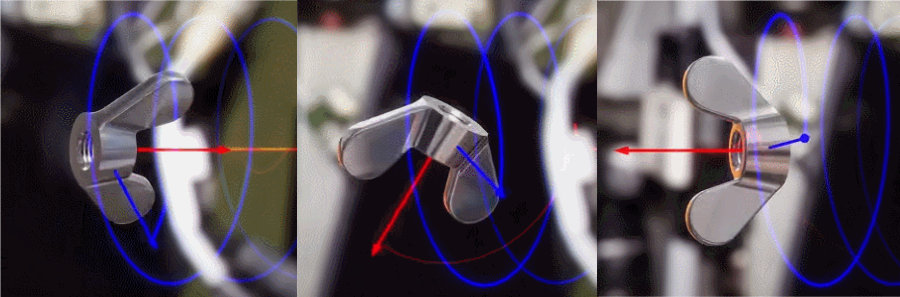
\includegraphics[width=0.9\textwidth]{dzhani.jpg}
\end{center}
   \caption{ภาพแสดงปรากฏการณ์ Dzhanibekov \cite{28}.}
\label{fig:10}
\end{figure*}

หลักการเบื้องหลังการเปลี่ยนแปลงแกนหมุนของโลกอย่างรวดเร็ว อยู่ที่ฟิสิกส์ของวัตถุหมุน ตัวอย่างมาตรฐานคือปรากฏการณ์ Dzhanibekov ซึ่งค้นพบโดยนักบินอวกาศชาวรัสเซีย Vladimir Dzhanibekov \cite{37} และแสดงในรูปที่ \ref{fig:10} วัตถุที่ไม่ได้หมุนอย่างสมบูรณ์แบบบนหนึ่งในสามแกนโมเมนต์ความเฉื่อยหลักจะไม่สามารถรักษาแกนหมุนไว้คงที่ได้ หากมันหมุนใกล้กับแกนที่สอง จะเกิดการเปลี่ยนแปลงทิศทางหมุนอย่างฉับพลัน แม้จะไม่ตรงกับสิ่งที่เชื่อว่าเกิดขึ้นในขณะโลกกลับแกนแบบฉับพลัน แต่อย่างน้อยในกรณีที่ไม่มีแรงภายนอก ฟิสิกส์ของการหมุนเท่านั้นที่สามารถอธิบายการเปลี่ยนแปลงแกนหมุนของโลกอย่างรวดเร็วได้

เพื่อความแม่นยำ โลกแทบจะไม่ได้เกิดปรากฏการณ์ Dzhanibekov แบบเรียบง่ายและสม่ำเสมอ หากเป็นเช่นนั้น เราจะสามารถตรวจจับการเปลี่ยนแปลงแกนหมุนของโลกอย่างค่อยเป็นค่อยไปเมื่อเวลาผ่านไป ตรงกันข้าม เราเชื่อว่าโลกประสบกับการหยุดชะงักแบบฉับพลันเป็นช่วงๆ ในโครงสร้างทางกายภาพของมัน ส่งผลให้เกิดการแยกตัวระหว่าง "การหมุนชั้นนอก" (เปลือกโลก/แมนเทิล) และ "วัตถุหมุนชั้นใน" (แกนกลาง) ตามกฎการอนุรักษ์โมเมนต์เชิงมุม หากไม่มีแรงกระตุ้นจากภายนอก โลกจะไม่สามารถเปลี่ยนแกนหมุนอย่างทันทีทันใดได้ ดังนั้นการแยกระหว่างวัตถุหมุนชั้นในและชั้นนอกจึงเป็นหนึ่งในไม่กี่สิ่ง (นอกเหนือจากผลกระทบจากภายนอก) ที่อาจทำให้เกิดการกลับแกนหมุนอย่างรวดเร็วและรุนแรง

กระบวนการเฉพาะที่ขับเคลื่อนการหยุดชะงักภายในของโลก เชื่อว่าเป็นการเปลี่ยนสถานะในโครงสร้างของเหล็กที่เป็นองค์ประกอบหลักของแกนโลก (รูปที่ \ref{fig:11}) แกนในประกอบด้วยเหล็กที่มีโครงสร้างแบบ hexagonal close-packed (Fe) \cite{141} เมื่อ hcp-Fe นี้เปลี่ยนสถานะเป็นของเหลวที่มีสมบัติของโลหะ จะปลดปล่อยพลังงานจลน์และถูกเคลื่อนเข้าไปในแกนชั้นนอก การเปลี่ยนเฟสนี้ลดความสามารถในการนำแม่เหล็กของแกนกลาง ทำให้สนามแม่เหล็กโลกอ่อนตัวลง และปลดปล่อยความร้อน สร้างโครงสร้าง LLVP (large low-velocity shear province) (รูปที่ \ref{fig:12}) \cite{38} ในชั้นแมนเทิล และเพิ่มอุณหภูมิพื้นผิวโลกผ่านมหาสมุทรน้ำลึก ทั้งสองแนวโน้มถูกบันทึกไว้อย่างดีในศตวรรษหลัง ๆ และจะมีการกล่าวถึงในส่วนถัดไปของบทความนี้

\begin{figure*}[t]
\begin{center}
% \fbox{\rule{0pt}{2in} \rule{.9\linewidth}{0pt}}
\includegraphics[width=1\textwidth]{layers.jpg}
\end{center}
   \caption{ภาพแสดงกระบวนการภายในโลกที่นำไปสู่การพลิกกลับของ ECDO \cite{129}.}
\label{fig:11}
\end{figure*}


\begin{figure}[t]
\begin{center}
% \fbox{\rule{0pt}{2in} \rule{0.9\linewidth}{0pt}}
   \includegraphics[width=1\linewidth]{llvp.jpg}
\end{center}
   \caption{ภาพเชิงลึกของ LLVP ใต้แอฟริกาใต้ \cite{28}.}
\label{fig:12}
\label{fig:onecol}
\end{figure}


กระบวนการเดียวกันนี้ภายในโลก ซึ่งเกิดขึ้นในทิศทางตรงกันข้าม ยังเชื่อกันว่าเป็นตัวผลักดันให้เกิดการเปลี่ยนกลับสู่สภาวะการหมุนของโลกในรูปแบบปัจจุบันในเวลาไม่นานหลังจากการพลิกกลับเกิดขึ้น

\section{หลักฐานเกี่ยวกับการพลิกกลับของโลกที่ใกล้จะเกิดขึ้น}
There is strong reason to believe that we are on the brink of another Earth flip. A cataclysm has not occurred for several millennia, which is approximately the frequency with which these events seem to happen based on historical accounts and data. The strongest data supporting an impending flip comes from recent geomagnetic data, which indicates that the Earth's geomagnetic field has been weakening for approximately two thousand years. This weakening has been accelerating and has reached alarming rates in the last few decades.

Depicted in Figure \ref{fig:14} is the geomagnetic field of Earth in 1590 and 2025 \cite{125,126}. As shown in the figure, the field has weakened significantly.

Another metric for the weakening geomagnetic field is the position of the geomagnetic north pole (Figure \ref{fig:13}). Geomagnetic north has historically been located in the Canadian Arctic. However, it has been wandering slowly over the last several centuries, and accelerated significantly a few decades ago. It is now moving rapidly towards Russia at a rate of 55 kilometers per year \cite{124}.

\begin{figure*}[t]
\begin{center}
% \fbox{\rule{0pt}{2in} \rule{.9\linewidth}{0pt}}
\includegraphics[width=0.9\textwidth]{saa.jpg}
\end{center}
   \caption{ภาพแสดงสนามแม่เหล็กโลกที่อ่อนตัวลงตั้งแต่ปี 1590 ถึง 2025 คำนวณโดยใช้แบบจำลอง gufm1 และ IGRF-14 \cite{125,126}.}
\label{fig:14}
\end{figure*}

\begin{figure}[t]
\begin{center}
% \fbox{\rule{0pt}{2in} \rule{1\linewidth}{0pt}}
   \includegraphics[width=1\linewidth]{npw.jpg}
\end{center}

\caption{ตำแหน่งของขั้วแม่เหล็กโลกเหนือ ตั้งแต่ปี 1590 ถึง 2025 แสดงในช่วงระยะเวลา 5 ปี \cite{142}.}
\label{fig:13}
\label{fig:onecol}
\end{figure}

\begin{figure}[t]
\begin{center}
% \fbox{\rule{0pt}{2in} \rule{1\linewidth}{0pt}}
   \includegraphics[width=1\linewidth]{ocean-highlight.jpg}
\end{center}
   \caption{อัตราการอุ่นขึ้นของมหาสมุทรส่วนลึก (ลึกกว่า 2000 เมตร) ตั้งแต่ปี 1991 ถึง 2010 ซึ่งถูกวงไว้ด้วยสีแดง \cite{132}.}
\label{fig:15}
\label{fig:onecol}
\end{figure}

สนามแม่เหล็กของโลกเชื่อว่าถูกสร้างขึ้นจากไดนาโมภายใน—กระแสแมกมาที่เคลื่อนที่เป็นเสาทรงกระบอกในแก่นนอกของโลกเนื่องมาจากการหมุนของโลก \cite{123}. การอ่อนกำลังของสนามแม่เหล็กโลกเป็นอาการของความปั่นป่วนลึกภายในโลก ตามทฤษฎี ECDO ความปั่นป่วนเหล่านี้จะทำให้เกิดการปล่อยความร้อน และในที่สุดนำไปสู่การแยกระหว่างแมนเทิลกับแก่นโลก ส่งผลให้เกิดการพลิกกลับของโลก \cite{1}.

มีข้อมูลจำนวนมากที่สนับสนุนการมีอยู่ของกระบวนการเกิดความร้อนภายในโลก ข้อมูลเกี่ยวกับโลกร้อนปรากฏในอุณหภูมิผิวทวีปและมหาสมุทรที่เพิ่มสูงขึ้น \cite{127,128} ระดับก๊าซคาร์บอนไดออกไซด์ในบรรยากาศที่เพิ่มขึ้นสัมพันธ์กับพลูมความร้อนของโลก \cite{129,130} และปริมาณน้ำแข็งทะเลทั่วโลกลดลง \cite{131}. ข้อมูลเหล่านี้ชี้ให้เห็นว่าระดับ CO2 และอุณหภูมิที่สูงขึ้นไม่ใช่สาเหตุของ “การเปลี่ยนแปลงสภาพภูมิอากาศที่มนุษย์สร้างขึ้น” แต่เป็นผลสืบเนื่องจากแก่นโลกที่ปล่อยความร้อนออกมา \cite{129}.

ที่สำคัญที่สุด การศึกษาอัตราการอุ่นขึ้นของมหาสมุทรส่วนลึก (ลึกกว่า 2000 เมตร) แสดงให้เห็นว่าไม่เพียงแต่มหาสมุทรส่วนลึกกำลังร้อนขึ้นแต่อัตราการอุ่นขึ้นที่แรงที่สุดพบในชั้นแอบิสซอล (4000 - 6000 เมตร) โดยศูนย์กลางของการอุ่นนี้อยู่ต่ำกว่า 4000 เมตร \cite{132,129} ซึ่งจะเป็นไปไม่ได้หากมหาสมุทรได้รับความร้อนจากด้านบนโดยบรรยากาศ ข้อมูลเช่นนี้สนับสนุนอย่างมากต่อแนวคิดที่ว่าการเปลี่ยนแปลงด้านภูมิอากาศและสนามแม่เหล็กโลกที่ผ่านมาในปัจจุบัน ขับเคลื่อนโดยกระบวนการที่อยู่ลึกภายในโลก รูปที่ \ref{fig:15} แสดงอัตราการอุ่นขึ้นของมหาสมุทรส่วนลึกทั่วโลก ตั้งแต่ปี 1991 ถึง 2010 \cite{132}.
\section{การสร้างแบบจำลองการพลิกกลับของโลกที่กำลังจะมาถึง}

\begin{figure}[b]
\begin{center}
% \fbox{\rule{0pt}{2in} \rule{1\linewidth}{0pt}}
   \includegraphics[width=1\linewidth]{saa-crop.jpeg}
\end{center}
   \caption{การคำนวณจุดพลิกผันโดยอิงจาก South Atlantic Anomaly ชี้ไปที่วันที่ 13 มีนาคม 2059 \cite{125,126}.}
\label{fig:16}
\label{fig:onecol}
\end{figure}

การคาดการณ์เวลาที่โลกจะพลิกกลับครั้งต่อไปเป็นงานที่ซับซ้อน ปัจจุบัน โมเดลที่ดีที่สุดที่เรามีสำหรับเรื่องนี้คือสนามแม่เหล็กโลก บริเวณ South Atlantic Anomaly (SAA) พื้นที่นี้ที่อยู่เหนือน่านน้ำแอตแลนติกใต้มีความเข้มสนามแม่เหล็กต่ำที่สุด และถูกกำหนดให้เป็นบริเวณที่มีค่าความเข้มของสนามต่ำกว่า 32,000 นาโนเทสลา \cite{135} ซึ่งเป็นค่าต่ำที่สุดที่เคยบันทึกไว้ในปี 1590 พื้นที่ของ South Atlantic Anomaly มีขนาดเพิ่มขึ้นจาก 1\% ของพื้นผิวโลกในปี 1590 เป็น 21\% ในปี 2025 \cite{136}

เพื่อประมาณการว่าโลกอาจจะพลิกกลับเมื่อใด ข้าได้ทำการปรับข้อมูลพื้นที่ผิวของ SAA ให้เข้ากับสมการ power-law tipping point ที่เป็นแบบจำลองของระบบซับซ้อนที่เข้าใกล้จุดเปลี่ยนวิกฤต ซึ่งระบบจะเกิดการเปลี่ยนแปลงอย่างรวดเร็วและรุนแรง การคำนวณของข้าให้วันที่จุดพลิกผันที่คาดการณ์ไว้คือวันที่ 13 มีนาคม 2059 (ดูรูป \ref{fig:16}) การคาดการณ์นี้จะมีความแม่นยำมากขึ้นเรื่อย ๆ เมื่อเราเข้าใกล้ช่วงเวลาแห่งการเปลี่ยนแปลง \cite{136}

ตัวชี้วัดอื่น ๆ เช่น การเคลื่อนที่ของแกนหมุนของโลก, ความผิดปกติของสภาพอากาศ, และข้อมูลแผ่นดินไหวกับภูเขาไฟ ก็สามารถช่วยให้เราคาดการณ์เวลาที่โลกจะพลิกกลับครั้งต่อไปได้แม่นยำยิ่งขึ้น

\section{เส้นเวลาเหตุการณ์สำคัญของ ECDO}
While establishing an exact timeline for past ECDO events is difficult, it seems that there were at least 2 ECDO events during the Holocene. Note the account told by Herodotus from Egyptian priests that, \textit{"ตั้งแต่กษัตริย์องค์แรกจนถึงมหาปุโรหิตแห่งเทพฮีฟีสทอสผู้ครองราชย์เป็นคนสุดท้าย ได้มีมนุษย์ถึงสามร้อยสี่สิบเอ็ดชั่วอายุคน... ในช่วงเวลานี้พวกเขากล่าวว่าดวงอาทิตย์ได้เคลื่อนตำแหน่งจากจุดขึ้นตามปกติถึงสี่ครั้ง และจุดที่มันตกในปัจจุบันเคยเป็นจุดที่มันขึ้นสองครั้ง และจุดที่มันขึ้นในปัจจุบันเคยเป็นจุดที่มันตกสองครั้ง"} \cite{32}. เพลโต ซึ่งมีชีวิตอยู่ในช่วงศตวรรษที่ห้าก่อนคริสต์ศักราช \cite{111} กล่าวว่าหลังจากน้ำท่วมที่จมแอตแลนติสภายในวันเดียว 9,000 ปีก่อน \textit{"ตั้งแต่นั้นเป็นต้นมาได้มีน้ำท่วมใหญ่หลายครั้ง และผู้รอดชีวิตที่พำนักอยู่บนภูเขาไม่รู้จักศิลปะแห่งการเขียน และในหลายชั่วอายุคนก็ทุ่มเทอย่างเต็มที่เพื่อการดำรงชีวิต"} \cite{112} ซึ่งบ่งชี้ว่าอาจมีการพลิกกลับมากกว่าสองครั้งตั้งแต่สิ้นสุดยุค Younger Dryas ประมาณ 9,700 ปีก่อนคริสต์ศักราช หลักฐานทางกายภาพที่นำเสนอตลอดบทความนี้และในการวิจัยของข้าพเจ้า \cite{2} ให้หลักฐานสนับสนุนบัญชีของเพลโตอย่างเพียงพอ

วันที่เป็นผู้สมัครล่าสุดสำหรับการพลิก ECDO คือช่วงปี 2300 ถึง 1600 ก่อนคริสต์ศักราช ซึ่งตำนานน้ำท่วมมหาภัยหลายกรณี (กัน-หยู่ \cite{113,114,115}, น้ำท่วมอ็อกกีส \cite{116,117}, เปรู \cite{118,119}, อพยพ \cite{120}), การล่มสลายและการละทิ้งอารยธรรม (โมเฮ็นโจ-ดาโร \cite{121}, ครีตไมโนอัน \cite{100,101}) และความผิดปกติทางกายภาพ (bond events \cite{122}, เหตุการณ์ 4.2 พันปี \cite{90}) ได้ถูกลงวันที่ ยังไม่มีหลักฐานมาบรรจบกันอย่างเพียงพอที่ใหม่กว่านี้ซึ่งชี้ให้เห็นถึงเหตุการณ์มหันตภัยใหญ่

\section{Conclusion}

ปฏิบัติการ NANOOK เป็นความพยายามลาดตระเวนในช่วงสงครามเย็นของสหรัฐอเมริกา เพื่อแผนที่ขั้วโลกเหนือและชายฝั่งโซเวียตตอนเหนือหลังสงครามโลกครั้งที่สอง \cite{137} ในระหว่างการสืบสวน พวกเขาค้นพบว่าเส้นแม่เหล็กโลกนั้นอยู่เหนือจุดที่ควรจะเป็นจากหลักฐานของการสำรวจยุคก่อนถึง 125 ถึง 200 ไมล์ ตามที่ระบุไว้ \textit{"ในหมู่นักวิทยาศาสตร์รัฐบาล จึงเกิดคำถามขึ้นมาว่าจะเกิดอะไรขึ้นเมื่อขั้วแม่เหล็กโลกกับขั้วทางภูมิศาสตร์มาตรงกัน เพื่อหาคำตอบนี้ ภายใต้การควบคุมโครงการของ ดร. พอล เอ. ไซเปิล บริษัทแรนด์คอร์ปอเรชั่นได้รับสัญญาให้ทำการทดลองในห้องปฏิบัติการโดยใช้แบบจำลองโลกที่สร้างจากทรงกลมซ้อนกัน – ทรงกลมด้านในแทนแกนเหล็กลาวาไฟฟ้าแม่เหล็กของโลกซึ่งระบุแกนและขั้ว “แม่เหล็ก” ; และทรงกลมด้านนอกแทนเปลือกโลกที่หมุนรอบแกนขั้ว “ภูมิศาสตร์” เมื่อทำซ้ำซ้อนการทดลอง ก็พบว่าเมื่อขั้ว “แม่เหล็ก” เคลื่อนเข้าใกล้ขั้ว “ภูมิศาสตร์” ขั้วแม่เหล็กจะเร่งความเร็วในการเคลื่อนเข้าใกล้อย่างรุนแรงเหมือนถูกดึงด้วยแรงเหวี่ยงเข้าสู่ขั้วภูมิศาสตร์และเคลื่อนไปตรงกันในที่สุด แต่แทนที่จะซ้อนตรงกัน ขั้ว “แม่เหล็ก” จะ “พลิก” อย่างรวดเร็วไปรอบขั้ว “ภูมิศาสตร์” และยิงออกไปทางเส้นศูนย์สูตรเหมือนกับแรงเหวี่ยง จนจบลงที่ตำแหน่งที่มุมสองแกนแยกกันประมาณ 89 องศา หลังการ “พลิก” ของขั้วนี้เกิดขึ้นแล้ว แกนทั้งสองจะเริ่มกลับเข้าหากันอย่างช้าๆ ตลอดเวลาที่ยาวนาน"} \cite{138,139}

ต่อมา \textit{"ที่การประชุมวิทยาศาสตร์ที่เมเจอร์ ไวท์เข้าร่วมหนึ่งในเพนตากอนช่วงต้นปี 1948 เหล่านักวิทยาศาสตร์ได้ถกเถียงกันถึงความเหมาะสมในการเตือนสาธารณชนเกี่ยวกับปรากฏการณ์ขั้วโลกพลิกกลับนี้ ไม่มีนักวิทยาศาสตร์คนใดเห็นควรจะปิดบังข้อมูลจากสาธารณะ แต่ในทางกลับกัน ก็ไม่มีใครตกลงกันได้ว่าจะเปิดเผยข้อมูลอย่างไร ความรู้นี้ บางคนคิดว่า อาจจะทำลายจิตวิญญาณทางจริยธรรมของสังคมด้วยซ้ำ ทว่าความกลัวนี้ดูจะไม่มีมูล เมื่อในต้นทศวรรษ 1950 ข้อมูลเกี่ยวกับปรากฏการณ์ขั้วโลกพลิกถูกเผยแพร่ทั้งในคอลัมน์หนังสือพิมพ์และบทความนิตยสาร แต่กลับไม่เกิดการตอบรับใด ๆ จากสาธารณชนที่ดูเหมือนจะตะลึงงันหรือไม่เชื่อ"} \cite{138,139}

ทำไมเราถึงไม่ใส่ใจกับเรื่องนี้? มีเหตุผลมากมายที่เชื่อว่าโลกเคยพลิกกลับมาก่อน บทความนี้ พร้อมกับภาคสองของบทความนี้ สรุปหลักฐานจำนวนมหาศาลจากหลากหลายแขนงที่บ่งชี้ว่าสิ่งนี้เป็นความจริง เช่น ตำนานน้ำท่วมทั่วโลก ฟอสซิลเกลือและทะเลที่ปกคลุมพื้นทวีป ที่หลบภัยใต้ดินโบราณ ซากสัตว์ และภูมิประเทศทางธรณีวิทยาที่เต็มไปด้วยอดีตภัยพิบัติ มนุษย์ว่าอายุหลายแสนปี แต่ประวัติศาสตร์สมัยใหม่ของเรามีแค่ไม่กี่พันปี อาจเป็นไปได้ไหมว่าทุก ๆ ระยะหนึ่ง โลกจะพลิกกลับ ทวีปถูกล้างจนเกลี้ยง แล้วเราก็ต้องกลับไปเริ่มต้นใหม่เหมือนยุคหิน ลดบันทึกประวัติศาสตร์โบราณเหลือเพียงเรื่องเล่าหายนะไม่กี่เรื่อง? หากเป็นเช่นนั้น การป้องกันไม่ให้มันเกิดขึ้นอีกก็อาจเป็นภารกิจสำคัญที่สุดของมนุษยชาติ

สุดท้ายนี้ ข้าพเจ้าขอฝากบัญชีเรื่องเล่าที่ถูกบันทึกไว้ใน Timaeus โดยเพลโต เกี่ยวกับการพูดคุยระหว่างโซลอน (Solon) นักการเมืองชาวเอเธนส์และนักบวชชาวอียิปต์ \cite{140}: \textit{"วันหนึ่ง เมื่อ [โซลอน] ต้องการชักชวนให้นักบวชสนทนาเรื่องประวัติศาสตร์โบราณ เขาเล่าขนบธรรมเนียมที่เก่าแก่ที่สุดของเราเกี่ยวกับฟอโรเนอุส (Phoroneus) ซึ่งเชื่อกันว่าเป็นมนุษย์คนแรก และนิโอเบ แล้วเขาก็เล่าตำนานเกี่ยวกับเดอูคาเลียนและพีร์รา (Deucalion and Pyrrha) หลังน้ำท่วม และว่าพวกเขารอดมาได้อย่างไร รวมถึงบอกสายตระกูลของลูกหลานพวกเขา และด้วยการบอกจำนวนปีที่เหตุการณ์เหล่านั้นเกิดขึ้น เขาพยายามคำนวณระยะเวลา โดยขณะนั้นนักบวชคนหนึ่งที่แก่ชรามากกล่าวขึ้นว่า “โอ้ โซลอน โซลอน ท่านกรีกทั้งหลายยังเป็นเด็กอยู่เสมอ ไม่เคยมีชาวกรีกคนใดแก่เลย” เมื่อได้ยินเช่นนี้เขาจึงถามว่า “ท่านหมายความว่าอย่างไร?” นักบวชจึงตอบว่า “พวกท่านยังเด็กในจิตวิญญาณ ทุกคนเลย เพราะว่าพวกท่านไม่มีความเชื่อหรือภูมิปัญญาใด ๆ ที่ได้รับตกทอดมาแต่โบราณ และไม่รู้วิทยาการใดที่เก่าแก่ จริง ๆ แล้วเหตุที่เป็นเช่นนี้ก็เพราะมีมหันตภัยพิฆาตมนุษยชาติมากมายเกิดขึ้น ซึ่งครั้งใหญ่ที่สุดคือไฟและน้ำ ส่วนที่น้อยกว่านั้นก็ด้วยเหตุอื่น ๆ อีกนับไม่ถ้วน เรื่องเล่าที่เล่าว่าในชาติของท่าน เช่นเดียวกับของเรา ว่าเมื่อก่อนฟาเอธอน (Phaethon) ลูกเฮลิออส ขับรถพระอาทิตย์ของบิดาแล้วขับไม่ได้ทางเดิมจนโลกถูกเผาทั้งหมด และเขาเองก็ตายด้วยสายฟ้านั้น แท้จริงแล้ว เรื่องนี้ฟังดูราวกับนิทาน แต่ความจริงคือมันเกิดจากการเปลี่ยนตำแหน่งของดวงดาวที่หมุนรอบโลก และการทำลายสิ่งต่าง ๆ บนโลกด้วยไฟรุนแรงซึ่งหมุนเวียนมาเป็นระยะ ๆ ช่วงเวลาเช่นนี้ คนที่บนภูเขาหรือที่สูงจะแย่กว่าคนที่อยู่ใกล้แม่น้ำหรือทะเล; สำหรับเรา แม่น้ำไนล์ ผู้ช่วยชีวิตในเรื่องอื่น ๆ ก็ช่วยเราในคราวนี้ด้วยโดยเอ่อสูงขึ้น ส่วนถ้าทวยเทพลงโทษโลกด้วยน้ำนอง คนเลี้ยงวัวเลี้ยงแกะบนภูเขารอด แต่คนในเมืองของท่านถูกกระแสน้ำพัดไปในทะเล ในแผ่นดินของเรา ไม่ว่าคราวนั้นหรือคราวใด น้ำก็ไม่ไหลบ่าจากฟ้า แต่จะผุดขึ้นจากใต้ดินด้วยซ้ำ ดังนั้น สิ่งที่ถูกอนุรักษ์ไว้ที่นี่จึงถือว่าเก่าแก่ที่สุดจริง ๆ ในทุกพื้นที่ที่ไม่มีร้อนหรือเย็นจัดยับยั้ง ย่อมมีมนุษย์เหลืออยู่เสมอมากบ้างน้อยบ้าง และถ้าเหตุการณ์ใดเกิดขึ้นยิ่งใหญ่สูงส่งหรือโดดเด่น ไม่ว่าจะที่นี่หรือที่ของท่านหรือที่อื่นใดที่เรารู้มา เรื่องเหล่านี้ถูกบันทึกไว้และเก็บรักษาในวิหารของเรา ส่วนชาวท่านและคนอื่น ๆ กลับต้องเริ่มต้นใหม่เสมอด้วยอักษรและศิลปะต่าง ๆ ทุกครั้งที่น้ำท่วมใหญ่จากฟ้ามาเยือน ก็จะเหลือแต่คนที่ไร้การศึกษา ท่านจึงกลับมาเป็นเด็กดังเดิม ไร้ความรู้ใด ๆ เกี่ยวกับสิ่งที่เกิดในอดีตทั้งในแดนนี้หรือของท่านแท้จริง เผ่าพันธุ์ที่ท่านเล่าเมื่อครู่นี้ โซลอน ก็ไม่ต่างอะไรกับนิทานเด็ก ๆ เพราะท่านจำได้แต่น้ำท่วมครั้งเดียว ทั้งที่เกิดมาหลายครั้งแล้ว อีกทั้งยังไม่รู้ว่าพันธุ์มนุษย์ที่สูงส่งที่สุดเกิดในแผ่นดินของท่านเอง ที่ซึ่งท่านและเมืองทั้งมวลในปัจจุบันของท่านถือกำเนิดมาจากเชื้อเล็ก ๆ ที่เหลือรอดมา แต่เรื่องนี้ก็เผลอเลือนไป เพราะรุ่นแล้วรุ่นเล่าผู้รอดชีวิตครั้งก่อนตายไปโดยไร้โอกาสเขียนบันทึก แต่ก่อนเกิดมหาหายนะจากน้ำ มหานครเอเธนส์ทุกวันนี้ได้ชื่อว่าเข้มแข็งที่สุดในสงครามและยอดเยี่ยมในทางอื่น ๆ งานศิลปะและการปกครองก็ยิ่งใหญ่ สิ่งใดที่เคยมีมายิ่งใหญ่เท่าไรเราเคยรับรู้"}.

นักบวชเหล่านี้แน่นอนว่าได้บอกโซลอนเกี่ยวกับอารยธรรมโบราณของแอตแลนติสด้วย: \textit{"ทุกสิ่งที่เรามีอยู่นี้ทั้งหมด ล้อมรอบปากทางที่เราเอ่ยถึง ก็คืออ่าวที่มีทางเข้าออกแคบ ๆ ส่วนข้างนอกคือมหาสมุทรที่แท้จริง และแผ่นดินที่ล้อมรอบย่อมเรียกขานว่าเป็นทวีปอย่างสมบูรณ์ ในเกาะแอตแลนติสนี้ มีพันธมิตรกษัตริย์ผู้มีอำนาจยิ่งใหญ่ปกครองเกาะและหลายเกาะรอบ ๆ ตลอดจนแผ่นดินนี้ถึงอียิปต์และจากยุโรปถึงทีเรนเนีย ให้ทั้งหมดรวมกันนี้เคยคิดจะยกพลตีประเทศของพวกเธอและเราและดินแดนทั้งหมดในช่องแคบ แต่ครั้งนั้นเอง ความกล้าหาญของรัฐเธอเปล่งประกายขึ้น รักษาเสรีภาพแก่ทุกผู้ทุกคน และในที่สุดเกิดแผ่นดินไหวกับน้ำท่วมร้ายแรงในวันหนึ่งคืนหนึ่ง กองทัพของพวกท่านและเกาะแอตแลนติสทั้งหมดจึงถูกกลืนหายไป"}.

\section{Acknowledgments}

ขอขอบคุณ Ethical Skeptic ผู้แต่งต้นฉบับวิทยานิพนธ์ ECDO สำหรับการทำวิทยานิพนธ์ที่ลึกซึ้งและบุกเบิกนี้จนสำเร็จ และแบ่งปันความรู้นี้กับโลก วิทยานิพนธ์ชุดสามส่วนของเขา \cite{1} ยังคงเป็นผลงานชิ้นเอกของทฤษฎี Exothermic Core-Mantle Decoupling Dzhanibekov Oscillation (ECDO) และมีข้อมูลมากมายเกี่ยวกับหัวข้อนี้มากกว่าที่ข้าพเจ้าได้กล่าวถึงโดยสังเขปที่นี่
ขอขอบคุณ Ankit ผู้ซึ่งได้ดำเนินการประมวลผลข้อมูลการรวบรวมเหตุการณ์หายนะในตารางที่ 1

และแน่นอน ขอบคุณยักษ์ใหญ่ผู้เป็นบ่าให้เรายืนอยู่; เหล่าผู้ที่ได้ทำการวิจัยและสืบค้นทุกอย่างที่ทำให้งานชิ้นนี้เป็นไปได้ และทำงานเพื่อส่องแสงให้แก่มนุษยชาติ

\clearpage
\twocolumn

\section{ภาพเพิ่มเติม}


\begin{figure}[H]
\begin{center}
% \fbox{\rule{0pt}{2in} \rule{1\linewidth}{0pt}}
   \includegraphics[width=1\linewidth]{wave.jpg}
\end{center}
   \caption{ดูใกล้ ๆ กับการกัดเซาะคลื่นแบบพาราโบลาและรอยเว้าด้านล่างที่พีระมิด Khafre \cite{27}.}
\label{fig:19}
\label{fig:onecol}
\end{figure}
\begin{figure}[H]
\begin{center}
% \fbox{\rule{0pt}{2in} \rule{1\linewidth}{0pt}}
   \includegraphics[width=1\linewidth]{star-stone.jpg}
\end{center}
   \caption{แผนที่ดวงดาวที่แกะสลักลงบนหินในปล่องหนึ่งของพีระมิดคูฟู \cite{28}.}
\label{fig:20}
\label{fig:onecol}
\end{figure}

\begin{figure*}[t]
\begin{center}
% \fbox{\rule{0pt}{2in} \rule{.9\linewidth}{0pt}}
\includegraphics[width=1\textwidth]{deepsea.jpg}
\end{center}
   \caption{ภาพแสดงความผิดปกติของความร้อนในมหาสมุทรลึกและช่วงก้นสมุทรเมื่อเทียบกับเส้นโค้งความร้อนในมหาสมุทรตามปกติจากชั้นบรรยากาศ ความผิดปกติของความร้อนโดยรวมได้มาจาก NOAA \cite{147} การกระจายความร้อนในระดับลึกและก้นสมุทรจากงานวิจัยของ Desbruyeres \cite{132} และการประมวลผลข้อมูลและการสร้างภาพโดย Ethical Skeptic \cite{129}.}
\label{fig:21}
\end{figure*}
\begin{figure*}[t]
\begin{center}
% \fbox{\rule{0pt}{2in} \rule{.9\linewidth}{0pt}}
\includegraphics[width=1\textwidth]{sealevel.jpeg}
\end{center}
   \caption{ระดับน้ำทะเลแสดงการเพิ่มขึ้นของความแปรปรวน 20\% ในระยะเวลา 75 ปี ที่สถานี 63 แห่ง บ่งชี้ถึงการเพิ่มขึ้นของความเร็วกระแสน้ำ การพุ่งขึ้นของความแปรปรวนระดับน้ำทะเลเกิดขึ้นพร้อมกับการพุ่งของคลื่นความร้อนในมหาสมุทร บ่งชี้ว่าทั้งสองอาจมีสาเหตุมาจากความร้อนจากส่วนลึกใต้มหาสมุทรของโลก \cite{2,129}.}
\label{fig:22}
\end{figure*}

\begin{figure*}[t]
\begin{center}
% \fbox{\rule{0pt}{2in} \rule{.9\linewidth}{0pt}}
\includegraphics[width=1\textwidth]{co2.jpg}
\end{center}
   \caption{ppm ของ CO2 ในบรรยากาศเพิ่มขึ้นอย่างต่อเนื่องในช่วง 45 ปีที่ผ่านมา มีแนวโน้มสาเหตุจากอุณหภูมิของมหาสมุทรที่เพิ่มขึ้น ที่มา: NOAA \cite{148,129}.}
\label{fig:23}
\end{figure*}

\begin{figure*}[t]
\begin{center}
% \fbox{\rule{0pt}{2in} \rule{.9\linewidth}{0pt}}
\includegraphics[width=1\textwidth]{ice.jpg}
\end{center}
   \caption{พื้นที่น้ำแข็งทะเลทั่วโลกได้ลดลงในช่วง 45 ปีที่ผ่านมา เนื่องจากโลกร้อนขึ้น แหล่งที่มา: ADS \cite{149}.}
\label{fig:24}
\end{figure*}

\clearpage
\twocolumn

{\small
\renewcommand{\refname}{เอกสารอ้างอิง}
\bibliographystyle{ieee}
\bibliography{egbib}
}

\end{document}